

\documentclass[11pt,a4paper,titlepage,oneside]{article}

\usepackage[most]{tcolorbox}
\usepackage{geometry}
\usepackage{hyperref} %links
\usepackage[document]{ragged2e} %floating text
\usepackage{helvet} %font
\usepackage{tocloft} % dots in table of contents sections


\usepackage{lipsum}
\usepackage{fancyhdr}


% hypthenationrules
\usepackage[T1]{fontenc}



\hypersetup{
    colorlinks,
    citecolor=black,
    filecolor=black,
    linkcolor=black,
    urlcolor=black
}
\urlstyle{same}



\geometry{
    a4paper,
    left=3cm,
    right=2.5cm,
    top=3cm,
    bottom=2.5cm
}

%remove random margin on side ? idk what happend
%\setlength{\oddsidemargin}{0pt}



%custom reusable colorbox rules
\newtcolorbox{simplebox}{colback=white, sharp corners, boxrule=1pt }


\renewcommand{\contentsname}{Sisällys} % override Contents => Sisallys on table of contents

\renewcommand{\familydefault}{\sfdefault} % set font



\renewcommand{\cftsecleader}{\cftdotfill{\cftdotsep}} % dots for sections


\def\filename{src/oppari.tex}




\newcommand\wordcount{
    \immediate\write18{texcount -sub=section \filename{} -inc  | grep Section | sed -e 's/+.*//' | sed -n \thesection p > 'count.txt'}
(\input{count.txt}words)}


\newcommand{\inputf}[1]{\def\filename{#1}\input{#1}}


\newcommand\filewcount{
    \immediate\write18{texcount -1 -sum \filename{} > count.txt }
    \input{count.txt} words }


% jos on testi definetty niin tee 
\newcommand{\istest}[2]{\ifx\testmode\undefined #2 \else #1 \fi}


% testi section näyttää word countin siltä sectionilta jos ei testi niin sitten näytä vain normaali section
\newcommand{\tsection}[2]{\istest{#1{#2\\} \wordcount \\ \medskip }{#1*{#2}}}


\newcommand{\pagesection}[1]{\istest{\section{#1}  }{\section*{#1}}}
\newcommand{\pagesubsection}[1]{\istest{\subsection{#1}  }{\subsection*{#1}}}


% adds page with everything
\newcommand{\addPage}[2]{
    \def\filename{#1}
    \pagesection{#2}
    \istest{ \filewcount \medskip }{}
    \input{#1}
}



% OPPARI SPESIFIC

\newcommand{\addPageOp}[2]{
    \def\filename{#1}
    \pagesubsection{#2}
    \istest{ \filewcount \medskip }{}
    \input{#1}
}

%lab citation style
\newcommand{\labcite}[1]{\setcitestyle{aysep={},open={(},close={.)}}\citep{#1}{}}

%lab citation style
\newcommand{\labciteend}[1]{\setcitestyle{aysep={},open={(},close={).}}\citep{#1}{}}

\newcommand{\labimgcite}[1]{\setcitestyle{aysep={},open={(},close={)}}\citep{#1}{}}

\newcommand{\hurl}[1]{\href{#1}{{\underline{\textcolor{blue}{#1}}}}}


% counter kuville
\newcounter{imgCounter}
\setcounter{imgCounter}{0}

\newcommand{\getImgCount}{
\addtocounter{imgCounter}{1}
\theimgCounter
}


% counter kaavioille
\newcounter{chartCounter}
\setcounter{chartCounter}{0}

\newcommand{\getChartCount}{
\addtocounter{chartCounter}{1}
\thechartCounter
}



\usepackage[finnish]{babel}
















% ------------------------------ BEGIN DOCUMENT ------------------------------ %
\begin{document}

\pagestyle{empty}


%------------------------------ COVER PAGE ------------------------------ %


\includegraphics[width=5cm,height=1cm]{./src/labimg.jpg}

\vspace{86mm}
\huge
\textbf{Kehityksen seuranta}
\newline

\large

\vspace{5mm}
\textbf{Oppimispäiväkirja}
\normalsize

\vspace{90mm}

LAB-ammattikorkeakoulu \newline
\vspace{2mm}
Tieto-ja tietolikenadsfklj, Insinööri (AMK) \newline
\vspace{2mm}
2024 \newline
\vspace{2mm}
Kimi Malkamäki

\newpage




%------------------------------ FIRST PAGE OF ABSTRACT ------------------------------ %
\begin{tabular}{ | l | }

    %hack for the tiivistelmä line
    \multicolumn{1}{l}{
        \begin{minipage}{6cm}
            \hspace{1mm}
            
        \end{minipage}
        \begin{minipage}{4.25cm}
            \hspace{1mm}
        \end{minipage}
        \begin{minipage}[t][1.95cm][t]{3.62cm}
            \large
            \textbf{ Tiivistelmä }
        \end{minipage}
    }\\

    \hline
    \begin{minipage}[b]{6cm}
        tekijä(t)
        \newline
        kimi malkamäki 
    \end{minipage}%
    % 2x2
    \begin{minipage}{8.5cm}
        \begin{tabular}{ | l | c | }
            \begin{minipage}[t][1cm][t]{4.25cm}
                julkaisun laji
                \newline
                Opinnäytetyö, AMK
            \end{minipage} & %
            %
            \begin{minipage}{3.62cm}
                valmistusaika
                \newline
                2024
            \end{minipage} \\ \hline%
            %
            \begin{minipage}[t][1cm][t]{4.25cm}
                sivumäärä
                \newline 
                xx+xx
            \end{minipage}
            &  \\ \hline
        \end{tabular}
    \end{minipage}%
    % end of 2x2
      \\ \hline

    \begin{minipage}[t][2cm][t]{8cm}
    Työn nimi 
        \newline 
    ammatissa kasvaminen 
        \newline 
    oppimispäiväkirja  
    \end{minipage}\\ \hline

    \begin{minipage}[t][1.5cm][t]{10cm}
    tutkinto ja koulutusala.\newline  tietoviestintätekniikka insinööri amk  

    \end{minipage}\\ \hline

    \begin{minipage}[t][7cm][t]{5cm}
    tiivistelmä: \newline lorem ipsim
    \end{minipage}\\ \hline

    \begin{minipage}[t][2cm][t]{5cm}
    avain sanat
    \end{minipage}\\ \hline

\end{tabular}

\newpage



% ------------------------------ SECOND PAGE OF ABSTRACT ------------------------------ %

tiivistelmä








\newpage


% ------------------------------ TABLE OF CONTENTS ------------------------------ %

%keep page numbers off
\setcounter{page}{0}
\pagestyle{empty}
\pagenumbering{gobble}

\tableofcontents





\newpage



% ------------------------------- TERMISTÖ ------------------------------- %


TERMISTÖ

mitä termejä käytetään


ECMAscript                  skriptaus-kieli standardi 


\newpage





% ------------------------------- CONTENT PRELUDE COMMANDS ------------------------------- %
%enable page counting
\pagenumbering{arabic}
\clearpage
\setcounter{page}{1}

%set heaader and footer
\pagestyle{fancy}
%%
\lfoot{}
\cfoot{}
\rfoot{}
%%
\lhead{}
\chead{}
\rhead{\thepage}
%%
\renewcommand{\headrulewidth}{0pt}
\renewcommand{\footrulewidth}{0pt}
%\newcommand{\n}{\newline\vspace{20mm}}


\section{Johdanto}              % ------------------------------- JOHDANTO ------------------------------- %


Opinnäytetyön tavoitteena on seurata kehittymistä 13 viikon seurantajakson aikana työharjoittelussa.
\medskip

jotain siitä että tämä on päiväkirja opinnäytetyö
ja seurantajaksolla on seurattu juttuja jne
\medskip

%shit
starttaamo on suomalainen startup, joka yrittää ratjoa ongelmia työ ergonomiaan, ja vähentää sairas loma päiviä, saamalla työntekijöitä liikkumaan.
\medskip






\newpage
\section{Lähtötilanne}         % ------------------------------- LÄHTÖTILANNE ------------------------------- %


ennen opinnäytetyön kirjoittamista ja seurantajakson alkamista. 

neljännen vuoden opiskelia

harrastuksena myös ohjelmointi

ei muuta työkokemusta alasta
\medskip

harjoitus jakson aikana opin juttuja ja sitä miten tehdä töitä työympäristössä









\newpage
\section{teoria}                % ------------------------------- TEORIA ------------------------------- %



\subsection{kehitys ympäristö / teknologia pino}

starttaamon käyttämä teknologia pino käyttää meteor, react, mongodb
näitä käyttämällä koko homma toimii





\subsection{Meteor}
tähän jotain meteorsita lorem ipsum

\subsubsection{Meteor metodit}





\newpage
\subsection{React}                % ------------------------------- REACT ------------------------------- %
\wordcount


\subsubsection{mikä on React}

%ei saa olla metatekstiä
%https://github.com/facebook/react/blob/main/README.md
%https://www.infoq.com/news/2013/06/facebook-react/
% molemmat siteerattu 27.5.24


% ei ole metan kehittämä vaan se on vaan ylläpitämä. facebookin työntekijä teki sen
React on metan kehittämä ja ylläpitämä avoimeen lähdekoodiin perustuva javascript kirjasto, joka on suunniteltu reaktiivisien käyttöliittyjien kehittämiseen.
%more text

%rnative selitys paremmin
reaktia voi käyttää web ja mobiili käyttöliittymien tekemiseen react nativella
%vitusti lisää tekstiä
\medskip








\subsubsection{jsx}

%https://react.dev/learn/writing-markup-with-jsx
%https://facebook.github.io/jsx/ 

% jsx = js xml
% https://medium.com/@sjarancio/what-is-jsx-e3dda0af3490

%transpilation
%https://www.scholarhat.com/tutorial/react/getting-started-with-jsx
% https://www.typescriptlang.org/docs/handbook/jsx.html

% kaikki viitattu 27.5

%html koodia uusiks
JSX (javascript XML) on sytaksi jatke javascriptille, joka antaa kehittäjän kirjoittaa html tyylistä koodia javascriptin sekaan
% asiakielellä
selain ei itse osaa lukea jsx koodia joten se pitää transpiloida javascriptiksi ennen kun sen voi deploy



% suora sitaatti https://facebook.github.io/jsx/ 
JSX ei ole ECMAscript standardissa, joten selaimet eivät osaa tulkita sitä, vaan JSX se on suunniteltu transpiloitavaksi johonkin ECMAscript standardia toteuttavalle kielelle
\medskip

\bigskip
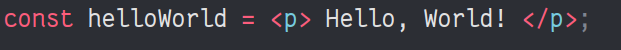
\includegraphics[width=10cm]{src/public/oppar/pure_jsx_example.png}

Kuva 1. kuvankaappaus JSX syntaxista.
\medskip

Kuvassa luodaan elementti helloWorld, jolle annetaan arvoksi paragraafi, jossa teksti "Hello, World!"{}.
% loppu pitää kirjottaa jotenkin paremmin ja pitää yhistää paremmin 
Elementtien arvot voidaan kirjoittaa html tyylillä, joka tekee jutuista kivaa.
\medskip



\bigskip

\includegraphics[width=15cm]{src/public/oppar/transpiled_jsx_example.png}

Kuva 2. Kuvankaappaus helloWorld elementistä, joka on käännetty javascriptiin. 
\medskip

%vähän toistoa muttei väliä sillä pitää siteerata tämä

%https://babeljs.io/repl 
kuvassa on helloworld elementti, joka on käännetty natiiviksi javascriptiksi babel kääntäjää käyttäen.
Tämä antaa selaimille mahdollisuuden tulkita JSX koodia.
%jotain lisää
\medskip

% https://github.com/facebook/react/blob/a4195750779dbd9a13e1615fbbd493bf2c5768ca/packages/react/src/ReactElement.js#L362
%pitää vissii kysyy voiko lähdekoodia käyttää lähteenä..


\subsubsection{Komponentit}


%https://react.dev/learn/your-first-component

Oma tekemä komponentti. se voi sisältää tilaa ja kutsuja muihin komponentteihin jne
komponentteihin voi lisätä interaktiivisuutta jne



komponentit on vähän niinkuin oma elementti jonkqa voi kirjoittaa jsx koodiin siististi

\medskip

\subsubsection{Reaktin struktuuri}
index.js lähtien
reactdom createroot
root.render
käy läpi kaikki lapset mitkä kaikilla componenteilla on ja tekee niistä natiivi html elementtejä jotka sitten selain renderöi. 

koko react läpi jsx kooditsta htmllään
\medskip



\subsubsection{VDOM}


%jotain domista, mikä se on ja miten se liittyy käyttöliittymiin ja sitten mikä on vdom
% vai pitäisikö samantien aloittaa että meillä on vdom, ja sittem selittää mikä dom on..... kuulostaa väärältä

virtuaali dom (document object model) on virtuaali representaatio oikeasta domista, 
dom on puu mainen struktuuri koko dokumentista


%https://medium.com/@BharathkumarV/reacts-virtual-dom-17fdcb290a10
% siteerattu 27.5

%selittää vähän paremmin ja tuntuu että puu struktuurinen ei ole oikein hyvä tapa kuvata domia
DOM (eng Document object model) on puu-struktuurinen representaatio koko käyttöliittymästä.
Tätä struktuuria käytetään rajapintana javascriptin ja html:län välillä. jotain jotain hidas.
%
VDOM (eng Virtual Dom) on virtuaalinen esitys domista jonka react pitää musitissaan koko suorituksen ajan.
vdomia käyttäen react voi nopeasti päätellä mitkä osat käyttöliittymästä pitää päivittää.
kun jonkun komponentin tila päivittyy react voi päivittää 






\newpage
\subsection{Mongodb}

jotain nosql mutta suurimmaksi osaksi mongodb tietokannasta






\subsection{Responsiiviset käyttöliittymät}
responsiivinen käyttöliittymän kehitys lorem ipsum






\subsection{Localisaatio}
lorem

\subsubsection{i18n}
en tiedä saanko hirveesti kirjotatteu
jos en niin kaada tämä ylempään
tai jos ei tule toista subsub sectionia










\newpage
\section{Toteutus}              % ------------------------------- TOTEUTUS ------------------------------- %


\subsection{Localisaatio}
localisaatio riippuen 


\subsection{Uuden ominaisuuden lisäys}
ipsum feature lisäys



\section{Yhteenveto}


sehän meni ihan hyvin 




\newpage
\section{Lähteet}               % ------------------------------- LÄHTEET ------------------------------- %

miten laitan liitteen päiväkirjasta ja millainen se pitäisi olla





\end{document}



